%%%%%%%%%%%%%%%%%%%%%%%%%%%%%%%%%%%%%%%%%
% Beamer Presentation
% LaTeX Template
% Version 1.0 (10/11/12)
%
% This template has been downloaded from:
% http://www.LaTeXTemplates.com
%
% License:
% CC BY-NC-SA 3.0 (http://creativecommons.org/licenses/by-nc-sa/3.0/)
%
%%%%%%%%%%%%%%%%%%%%%%%%%%%%%%%%%%%%%%%%%

%----------------------------------------------------------------------------------------
%	PACKAGES AND THEMES
%----------------------------------------------------------------------------------------

\documentclass{beamer}

\mode<presentation> {

% The Beamer class comes with a number of default slide themes
% which change the colors and layouts of slides. Below this is a list
% of all the themes, uncomment each in turn to see what they look like.

%\usetheme{default}
%\usetheme{AnnArbor}
%\usetheme{Antibes}
%\usetheme{Bergen}
%\usetheme{Berkeley}
%\usetheme{Berlin}
%\usetheme{Boadilla}
%\usetheme{CambridgeUS}
%\usetheme{Copenhagen}
%\usetheme{Darmstadt}
%\usetheme{Dresden}
%\usetheme{Frankfurt}
%\usetheme{Goettingen}
%\usetheme{Hannover}
%\usetheme{Ilmenau}
%\usetheme{JuanLesPins}
%\usetheme{Luebeck}
\usetheme{Madrid}
%\usetheme{Malmoe}
%\usetheme{Marburg}
%\usetheme{Montpellier}
%\usetheme{PaloAlto}
%\usetheme{Pittsburgh}
%\usetheme{Rochester}
%\usetheme{Singapore}
%\usetheme{Szeged}
%\usetheme{Warsaw}

% As well as themes, the Beamer class has a number of color themes
% for any slide theme. Uncomment each of these in turn to see how it
% changes the colors of your current slide theme.

%\usecolortheme{albatross}
%\usecolortheme{beaver}
%\usecolortheme{beetle}
%\usecolortheme{crane}
%\usecolortheme{dolphin}
%\usecolortheme{dove}
%\usecolortheme{fly}
%\usecolortheme{lily}
%\usecolortheme{orchid}
%\usecolortheme{rose}
%\usecolortheme{seagull}
%\usecolortheme{seahorse}
%\usecolortheme{whale}
%\usecolortheme{wolverine}

%\setbeamertemplate{footline} % To remove the footer line in all slides uncomment this line
%\setbeamertemplate{footline}[page number] % To replace the footer line in all slides with a simple slide count uncomment this line

%\setbeamertemplate{navigation symbols}{} % To remove the navigation symbols from the bottom of all slides uncomment this line
}

\usepackage{graphicx} % Allows including images
\usepackage{booktabs} % Allows the use of \toprule, \midrule and \bottomrule in tables

%----------------------------------------------------------------------------------------
%	TITLE PAGE
%----------------------------------------------------------------------------------------

\title[social and financial interactions]{Interplay between social and financial interactions in a crypto-currency } % The short title appears at the bottom of every slide, the full title is only on the title page

\author{\textbf{Nicolas Gensollen}, Matthieu Latapy} % Your name
\institute[LIP6] % Your institution as it will appear on the bottom of every slide, may be shorthand to save space
{
Laboratoire d'informatique de Paris 6 \\ % Your institution for the title page
\medskip
\textit{nicolas.gensollen@lip6.fr \\
\bigskip
MARAMI 2019 - Dijon - France} % Your email address
}
\bigskip
\date{November 6, 2019} % Date, can be changed to a custom date

\begin{document}

\begin{frame}
\titlepage % Print the title page as the first slide
\end{frame}

\begin{frame}
\frametitle{Overview} % Table of contents slide, comment this block out to remove it
\tableofcontents % Throughout your presentation, if you choose to use \section{} and \subsection{} commands, these will automatically be printed on this slide as an overview of your presentation
\end{frame}

%----------------------------------------------------------------------------------------
%	PRESENTATION SLIDES
%----------------------------------------------------------------------------------------


%------------------------------------------------
\section{Context} 
%------------------------------------------------

\begin{frame}
\Huge{\centerline{Context}}
\end{frame}


%------------------------------------------------
\subsection{Who are we?}
%------------------------------------------------

\begin{frame}
	\frametitle{\textbf{Who} we are and \textbf{what} we do}
	\only<1>{{\Large \textbf{The team}}}
	\onslide<2-3>{{\Large \textbf{Our main research topics}}}
	\only<2>{\\ \bigskip \textbf{Stream Graphs} \footnote{{\footnotesize \textit{Stream Graphs and Link Streams for the Modeling of Interactions over Time} Matthieu Latapy, Tiphaine Viard and Clémence Magnien Social Networks Analysis and Mining, 8: 61, 2018}}}
	\only<3>{\\ \bigskip \textbf{Anomaly detection}}
	\begin{center}
		\only<1>{
		\begin{itemize}
			\item \textit{Complex Networks} team (LIP6).
			\item Internet measurements, random graphs, temporal networks
			\item Social network analysis, spreading phenomena, graph algorithms
		\end{itemize}
		\bigskip
		\begin{figure}
			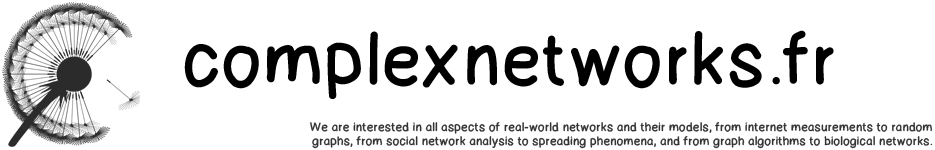
\includegraphics[width=\linewidth]{./figures/header}
		\end{figure}	
		}
		\only<2>{
		\bigskip
		\begin{figure}
			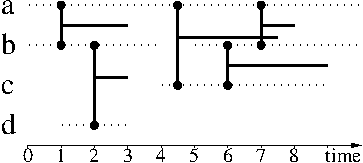
\includegraphics[width=.8\linewidth]{./figures/stream_graph}
		\end{figure}
		}
		\only<3>{
		\bigskip
		\begin{figure}
			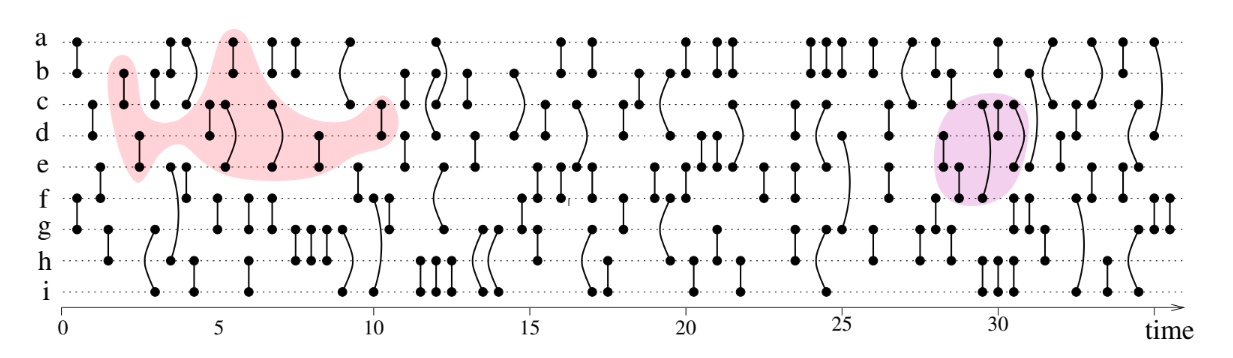
\includegraphics[width=\linewidth]{./figures/anomalie_detection}
		\end{figure}
		}
	\end{center}
\end{frame}


%------------------------------------------------
\subsection{The $\tilde{G}1$ crypto-currency}
%------------------------------------------------

\begin{frame}
	\frametitle{The $\tilde{G}1$ crypto-currency - \textbf{Transactions}}
	\onslide<1->{\textbf{Enables transactions between members}}
	\medskip
	\only<2>{\\{\small A transaction $\left(t,u,v\right) $: \textit{Entity $u$ sends money to entity $v$ at time $t$}.\\Transaction link stream: $ \mathcal{T} = \left( T, V, E_{\mathcal{T}} \right) $}}
	\only<3>{
		\begin{center}
			$T = \left[0,5\right]$, $V = \left\{a,b,c,d\right\}$
		\end{center}
	}
	\only<4>{
		\begin{center}
			No dynamics on the nodes
		\end{center}
	}
	\only<5>{
		\begin{center}
			$\left(0,c,b\right)$
		\end{center}
	}
	\only<6>{
		\begin{center}
			$\left(1,a,b\right),\left(1,d,c\right)$
		\end{center}
	}
	\only<7>{
		\begin{center}
			$\left(2,d,a\right)$
		\end{center}
	}
	\only<8>{
		\begin{center}
			$\left(4,a,d\right),\left(4,b,a\right)$
		\end{center}
	}
	\only<9>{
		\begin{center}
			$\left(5,b,a\right),\left(5,b,c\right)$
		\end{center}
	}
	\only<10>{
		\begin{center}
			$E_{\mathcal{T},1}=\left\{ \left(a,b\right), \left(d,c\right) \right\}$
		\end{center}
	}
	\only<11>{
		\begin{center}
			$E_{\mathcal{T},3}=\emptyset$
		\end{center}
	}
	\begin{center}
		\begin{figure}
			\only<3>{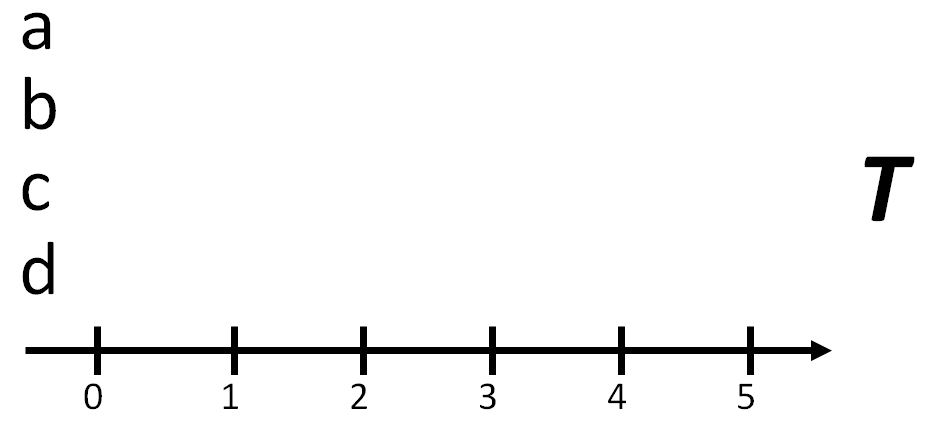
\includegraphics[width=\linewidth]{./figures/animation_transaction/transaction-0}}
			\only<4>{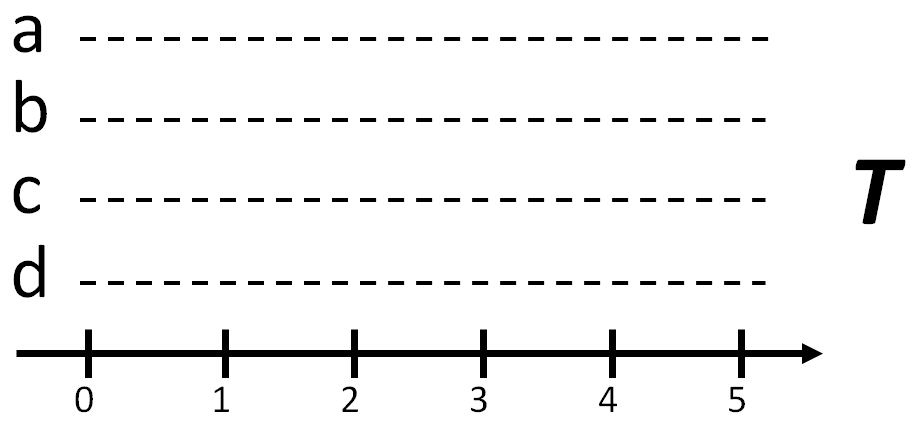
\includegraphics[width=\linewidth]{./figures/animation_transaction/transaction-1}}
			\only<5>{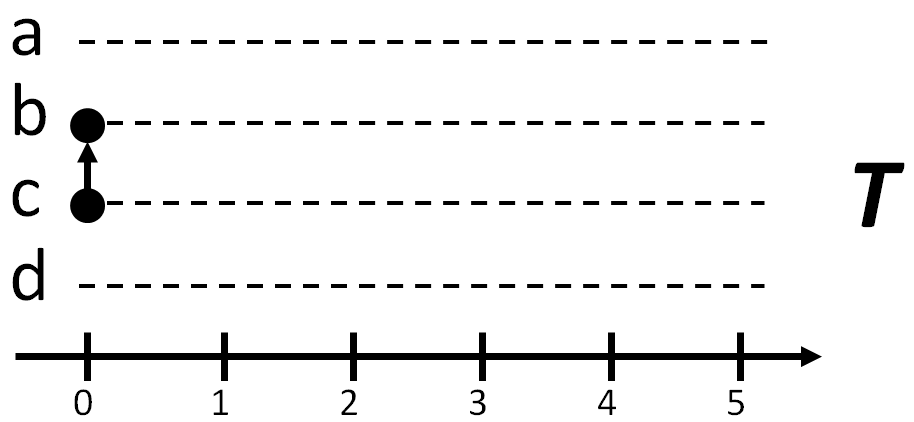
\includegraphics[width=\linewidth]{./figures/animation_transaction/transaction-2}}
			\only<6>{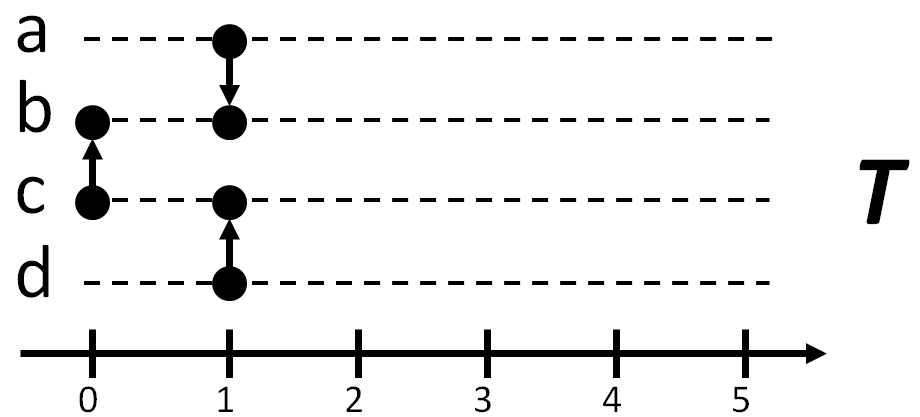
\includegraphics[width=\linewidth]{./figures/animation_transaction/transaction-3}}
			\only<7>{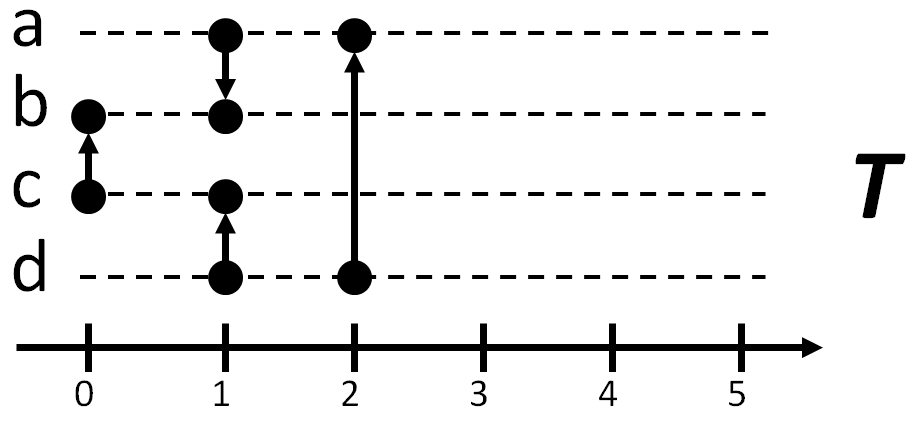
\includegraphics[width=\linewidth]{./figures/animation_transaction/transaction-4}}
			\only<8>{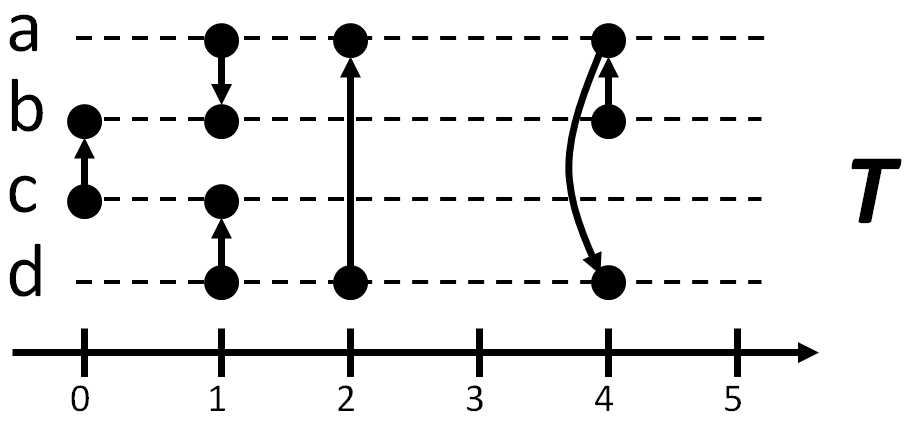
\includegraphics[width=\linewidth]{./figures/animation_transaction/transaction-5}}
			\only<9>{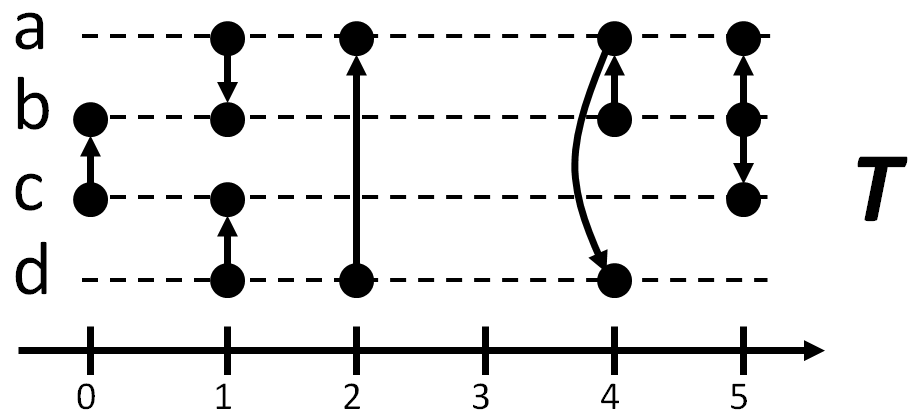
\includegraphics[width=\linewidth]{./figures/animation_transaction/transaction-6}}
			\only<10>{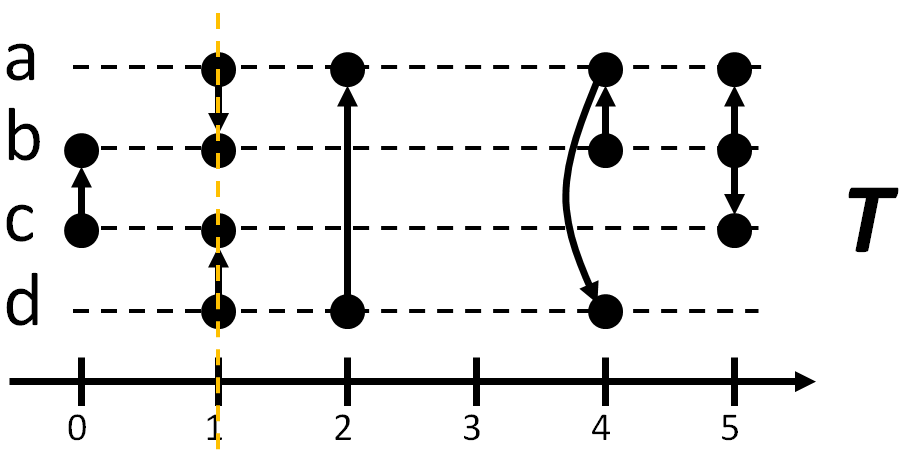
\includegraphics[width=\linewidth]{./figures/animation_transaction/transaction-7}}
			\only<11>{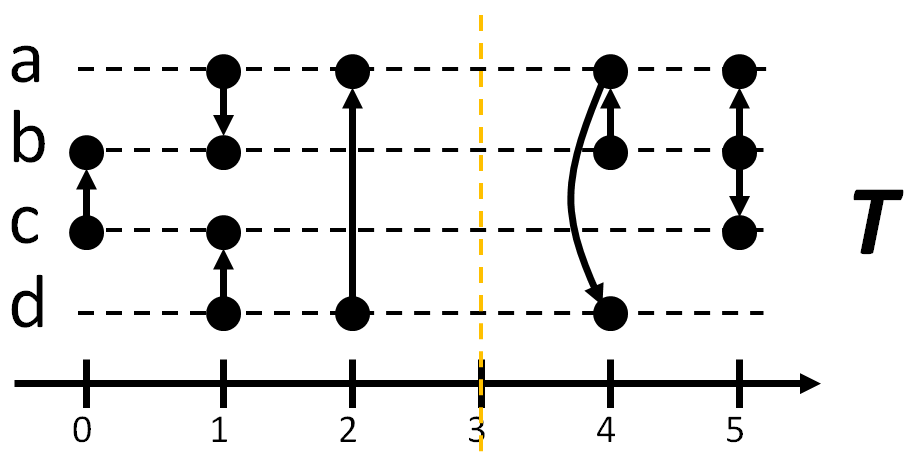
\includegraphics[width=\linewidth]{./figures/animation_transaction/transaction-8}}
		\end{figure}
	\end{center}
\end{frame}

%------------------------------------------------

\begin{frame}
	\frametitle{The $\tilde{G}1$ crypto-currency - \textbf{Certifications}}
	\onslide<1->{\textbf{Identification of the members with a Web of Trust mechanism}}
	\medskip
	\only<2>{\\{\small A certification $\left(t,u,v\right) $: \textit{Member $u$ certifies identity of member $v$ at time $t$}.\\Certification link stream: $ \mathcal{C} = \left( T, V, E_{\mathcal{C}} \right) $}}
	\only<3>{
		\begin{center}
			$T = \left[0,5\right]$, $V = \left\{a,b,c,d\right\}$
		\end{center}
	}
	\only<4>{
		\begin{columns}
		\column{.5\textwidth}
			\begin{center}
				$\left(0,b,c\right)$
			\end{center}
		\column{.5\textwidth}
			\begin{center}
				\begin{figure}
					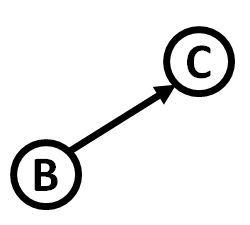
\includegraphics[width=.2\linewidth]{./figures/animation_wot/wot-1}
				\end{figure}
			\end{center}
		\end{columns}
	}
	\only<5>{
	\begin{columns}
	\column{.5\textwidth}
		\begin{center}
			$\left(2,a,b\right)$
		\end{center}
	\column{.5\textwidth}
		\begin{center}
			\begin{figure}
				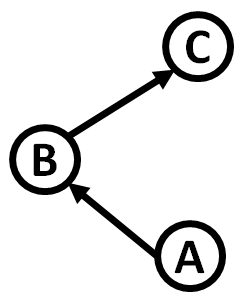
\includegraphics[width=.2\linewidth]{./figures/animation_wot/wot-2}
			\end{figure}
		\end{center}
	\end{columns}
	}
	\only<6>{
	\begin{columns}
	\column{.5\textwidth}
		\begin{center}
			$\left(3,d,a\right)$
		\end{center}
	\column{.5\textwidth}
		\begin{center}
			\begin{figure}
				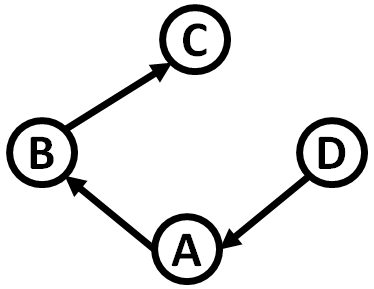
\includegraphics[width=.2\linewidth]{./figures/animation_wot/wot-3}
			\end{figure}
		\end{center}
	\end{columns}
	}
	\only<7>{
	\begin{columns}
	\column{.5\textwidth}
		\begin{center}
			$\left(4,d,c\right)$
		\end{center}
	\column{.5\textwidth}
		\begin{center}
			\begin{figure}
				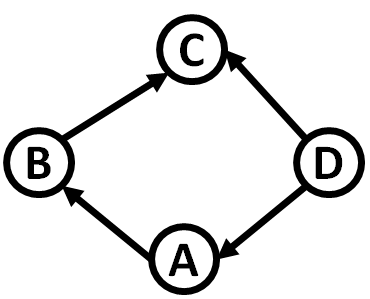
\includegraphics[width=.2\linewidth]{./figures/animation_wot/wot-4}
			\end{figure}
		\end{center}
	\end{columns}
		}
	\only<8>{
		\begin{center}
			$E_{\mathcal{C},1}=\left\{ \left(b,c\right) \right\}$
		\end{center}
	}
	\only<9>{
		\begin{center}
			$E_{\mathcal{C},5}=\left\{ \left(b,c\right),\left(a,b\right),\left(d,a\right),\left(d,c\right)\right\}$
		\end{center}
	}
	\begin{center}
		\begin{figure}
			\only<3>{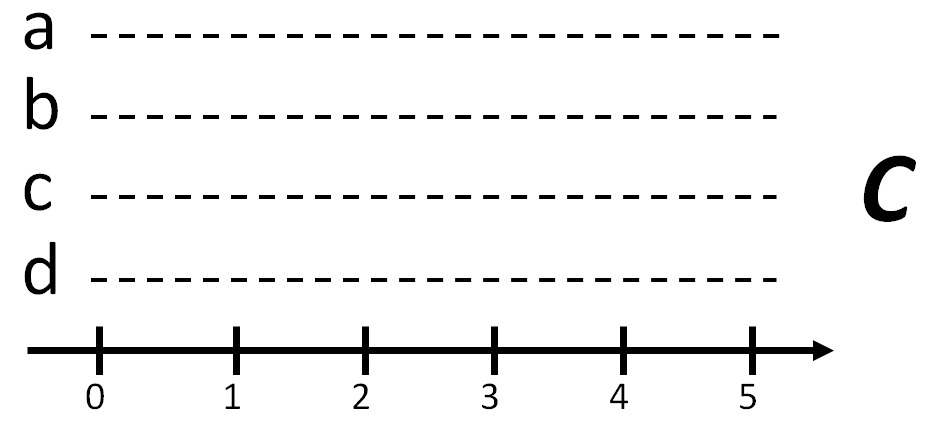
\includegraphics[width=\linewidth]{./figures/animation_certification/certification-0}}
			\only<4>{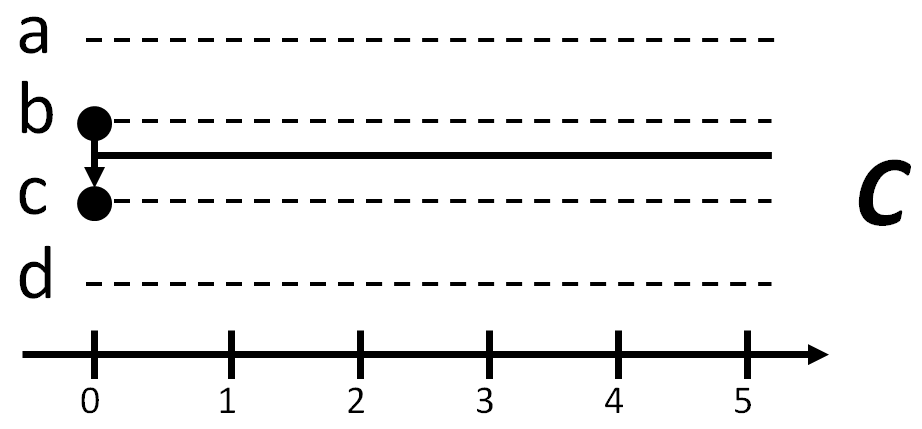
\includegraphics[width=\linewidth]{./figures/animation_certification/certification-1}}
			\only<5>{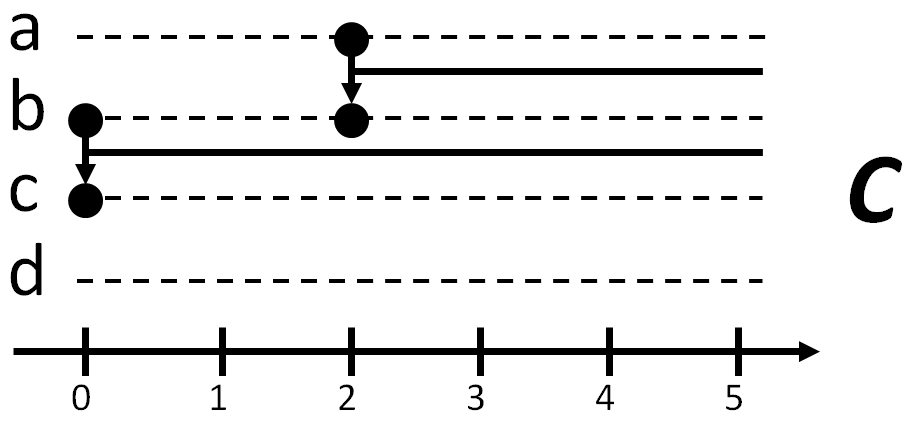
\includegraphics[width=\linewidth]{./figures/animation_certification/certification-2}}
			\only<6>{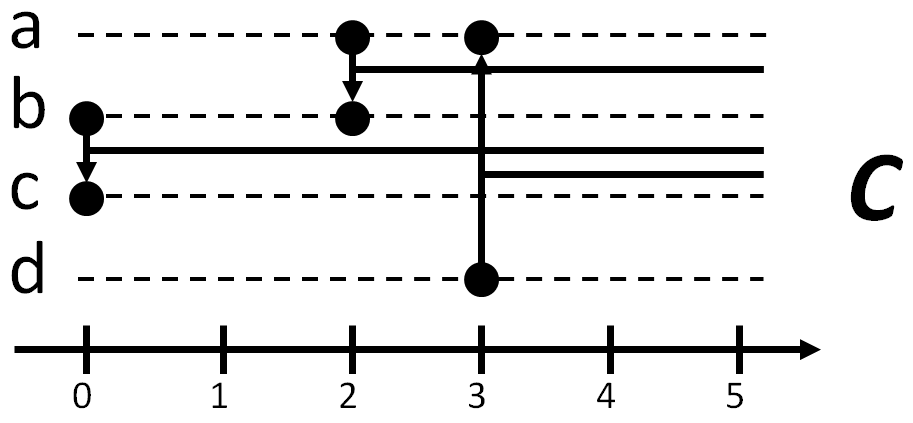
\includegraphics[width=\linewidth]{./figures/animation_certification/certification-3}}
			\only<7>{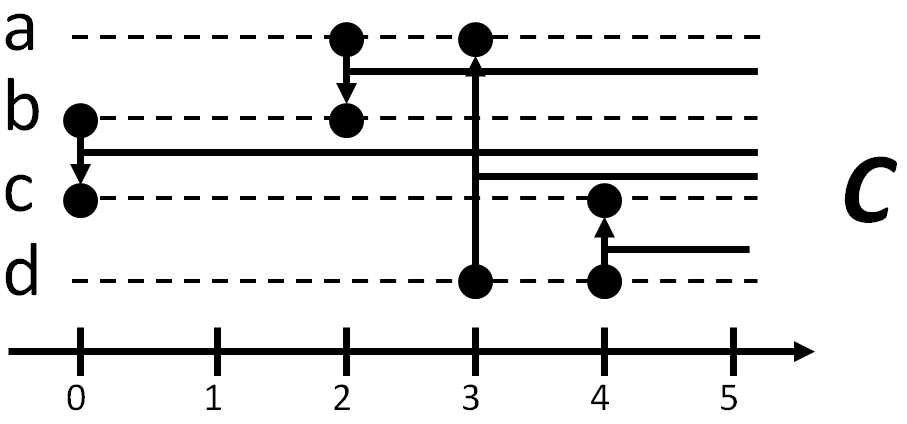
\includegraphics[width=\linewidth]{./figures/animation_certification/certification-4}}
			\only<8>{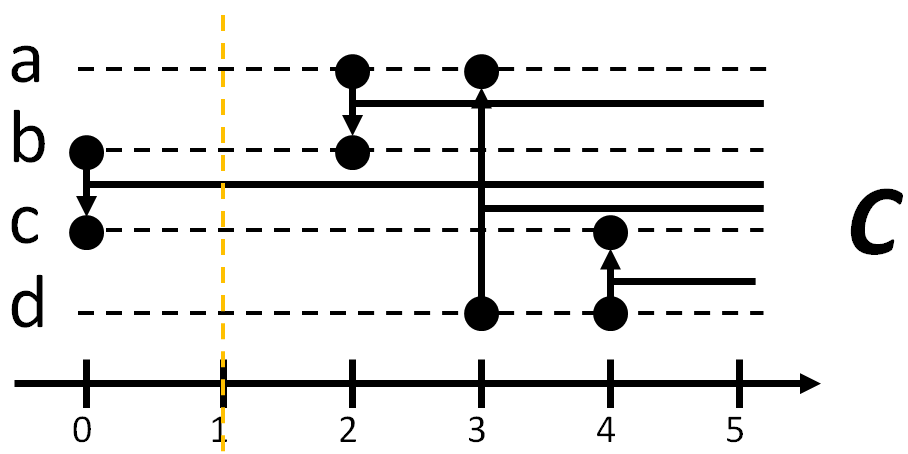
\includegraphics[width=\linewidth]{./figures/animation_certification/certification-5}}
			\only<9>{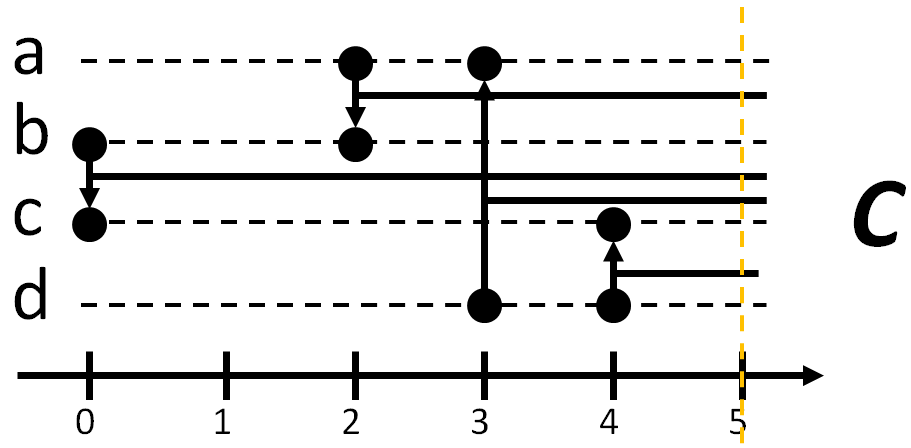
\includegraphics[width=\linewidth]{./figures/animation_certification/certification-6}}
		\end{figure}
	\end{center}	
\end{frame}

%------------------------------------------------

\begin{frame}
	\frametitle{Why is this great?}
	{\footnotesize We have a dynamic network of \textbf{social ties} and \textbf{financial transactions} between \textbf{identified human beings}!}
	\begin{center}
		\begin{figure}
			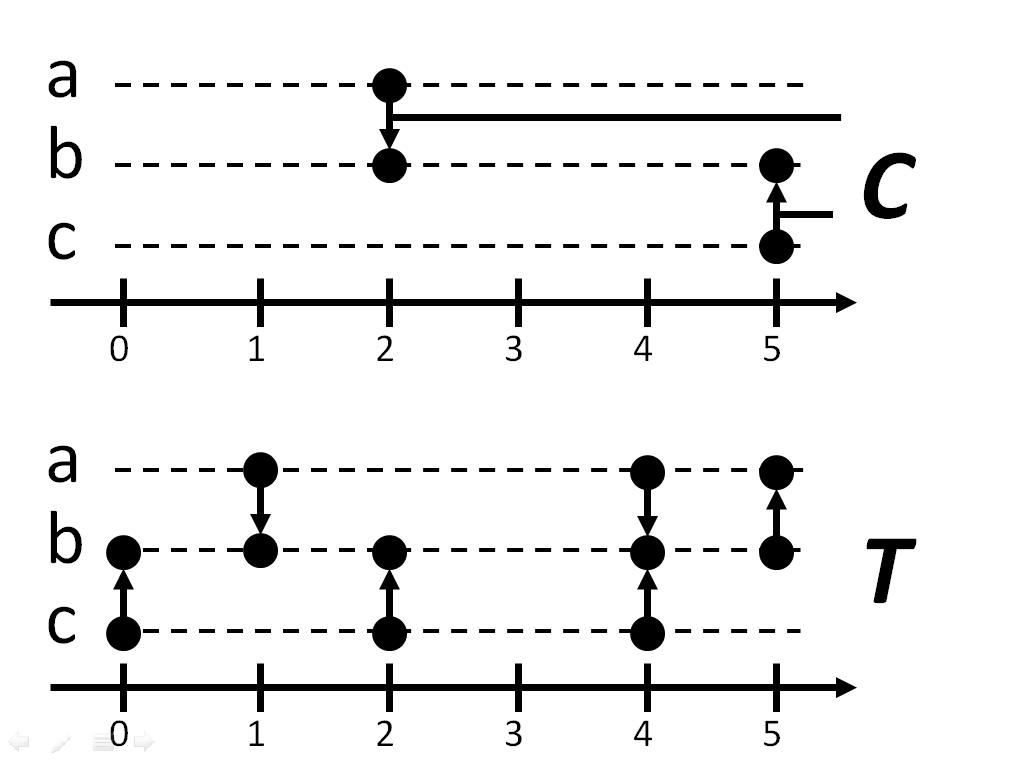
\includegraphics[width=.8\linewidth]{./figures/animation_dt/deltat-certif-0.png}
		\end{figure}
	\end{center}
\end{frame}


%------------------------------------------------
\section{Results}
%------------------------------------------------

%------------------------------------------------
\subsection{Time between Transactions and Certifications}
%------------------------------------------------

\begin{frame}
	\Huge{\centerline{Results}}
\end{frame}

%------------------------------------------------

\begin{frame}
	\frametitle{Time between transactions and certifications - \textbf{Questions}}
	{\Large \textbf{Questions:}}
	\bigskip
	\begin{itemize}
		\item<1-> If $a$ and $b$ are certified, did/will they make transactions? 
		\medskip
		\item<2-> How much time separate the certification from the closest matching transaction?
		\medskip
		\item<3-> If $a$ and $b$ make a new transaction, are/will they certify?
		\medskip
		\item<4-> How much time separate the transaction from the closest matching certification?
	\end{itemize}
\end{frame}


%------------------------------------------------

\begin{frame}
	\frametitle{Time between transactions and certifications - \textbf{Method}}
	\begin{center}
		\begin{figure}
			\only<1>{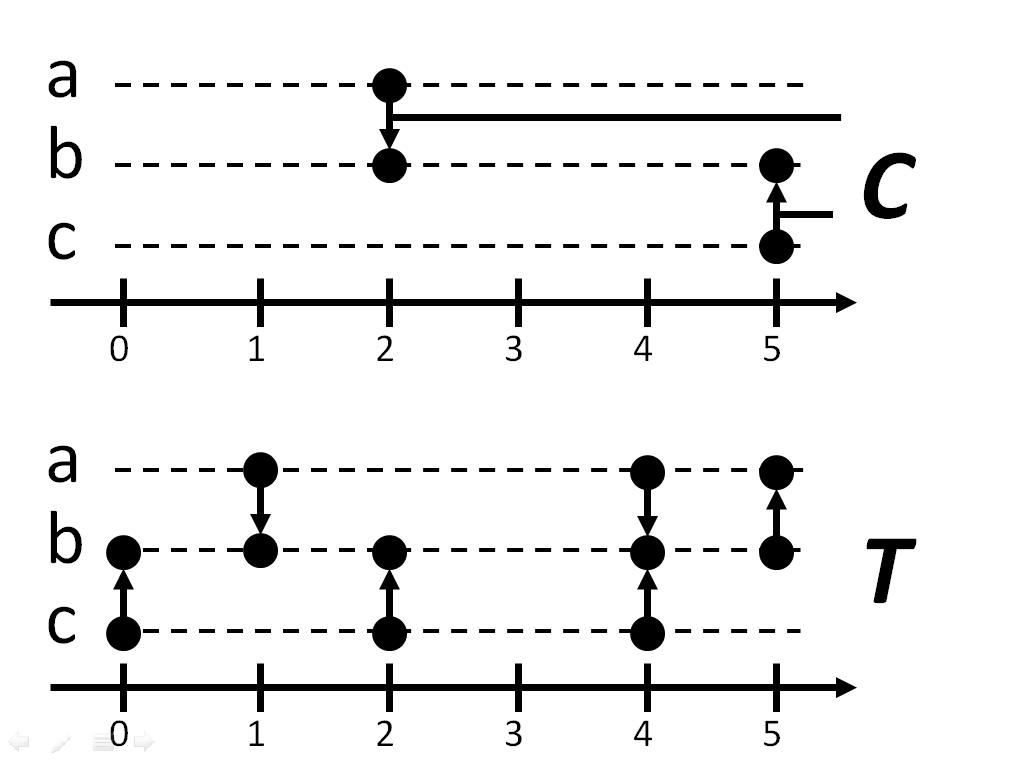
\includegraphics[width=.9\linewidth]{./figures/animation_dt/deltat-certif-0.png}}
			\only<2>{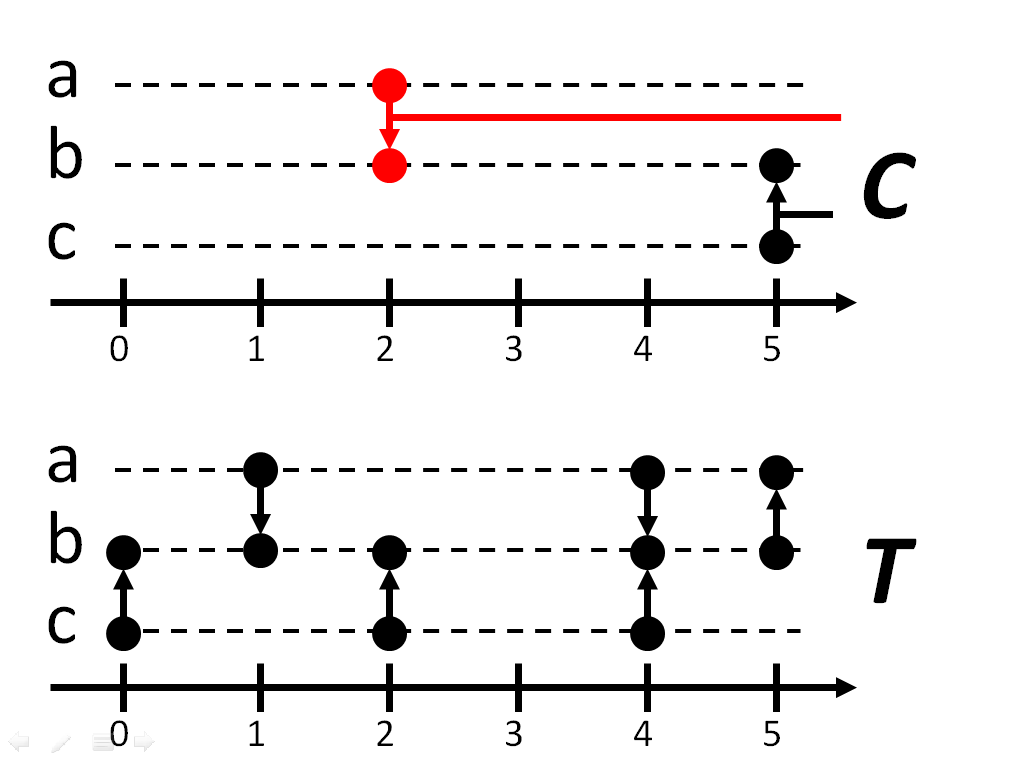
\includegraphics[width=.9\linewidth]{./figures/animation_dt/deltat-certif-1.png}}
			\only<3>{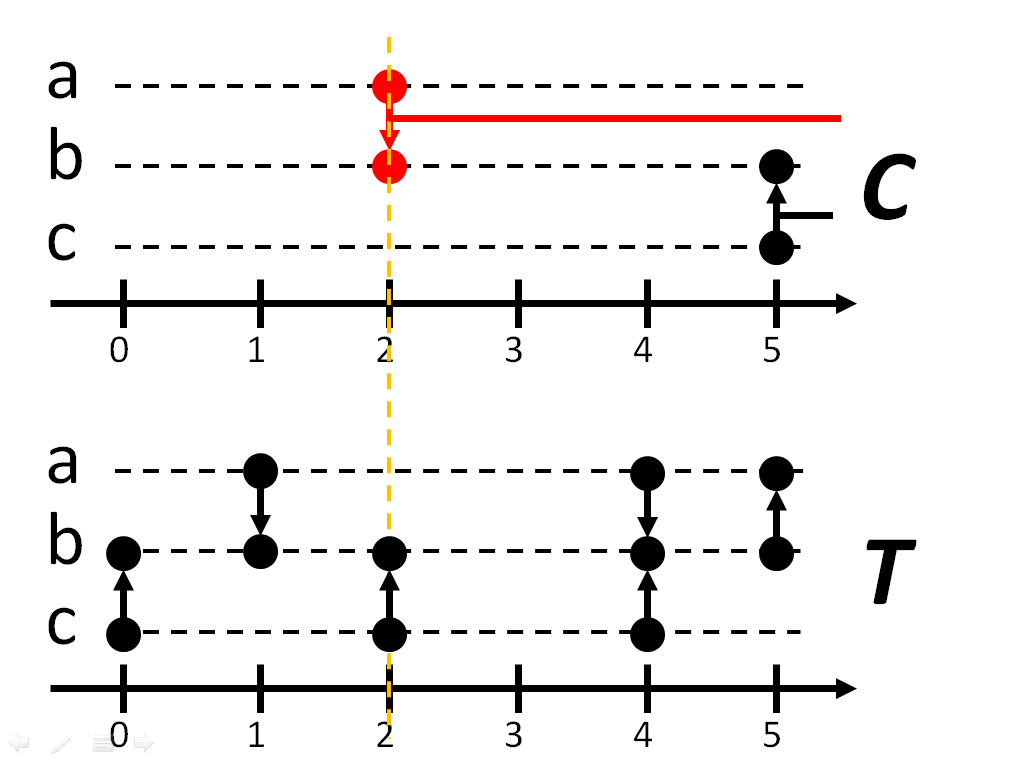
\includegraphics[width=.9\linewidth]{./figures/animation_dt/deltat-certif-2.png}}
			\only<4>{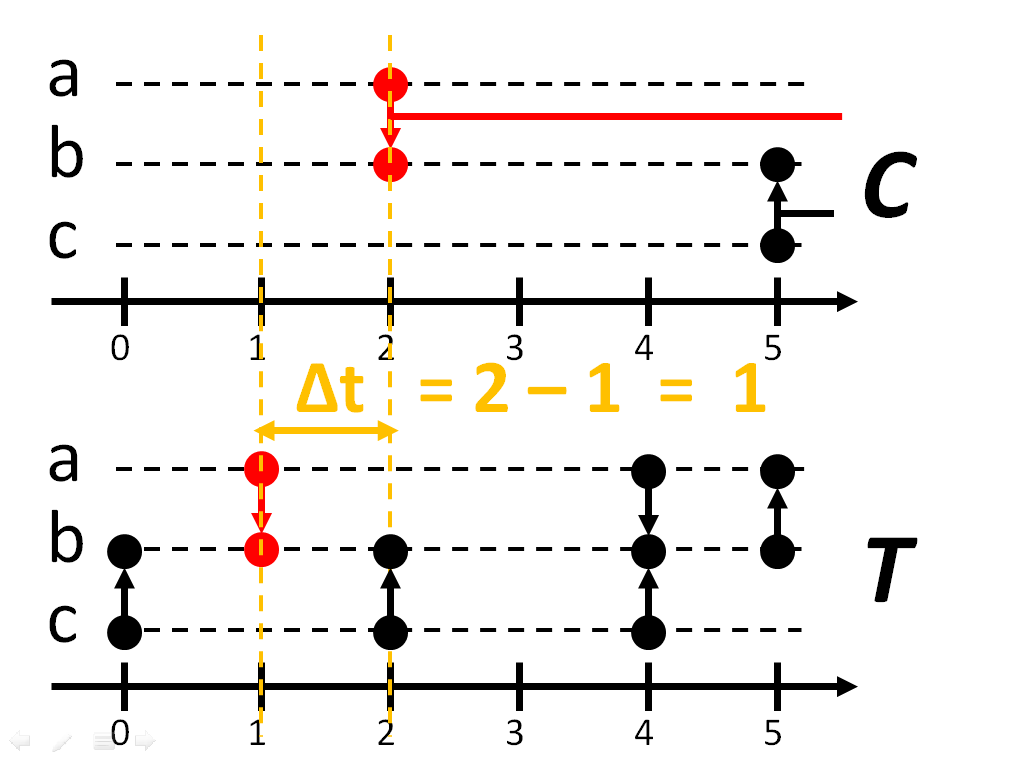
\includegraphics[width=.9\linewidth]{./figures/animation_dt/deltat-certif-3.png}}
		\end{figure}
	\end{center}
\end{frame}


%------------------------------------------------
	
\begin{frame}
	\frametitle{Time between transactions and certifications - \textbf{Method}}
	\begin{center}
		\begin{figure}
			\only<1>{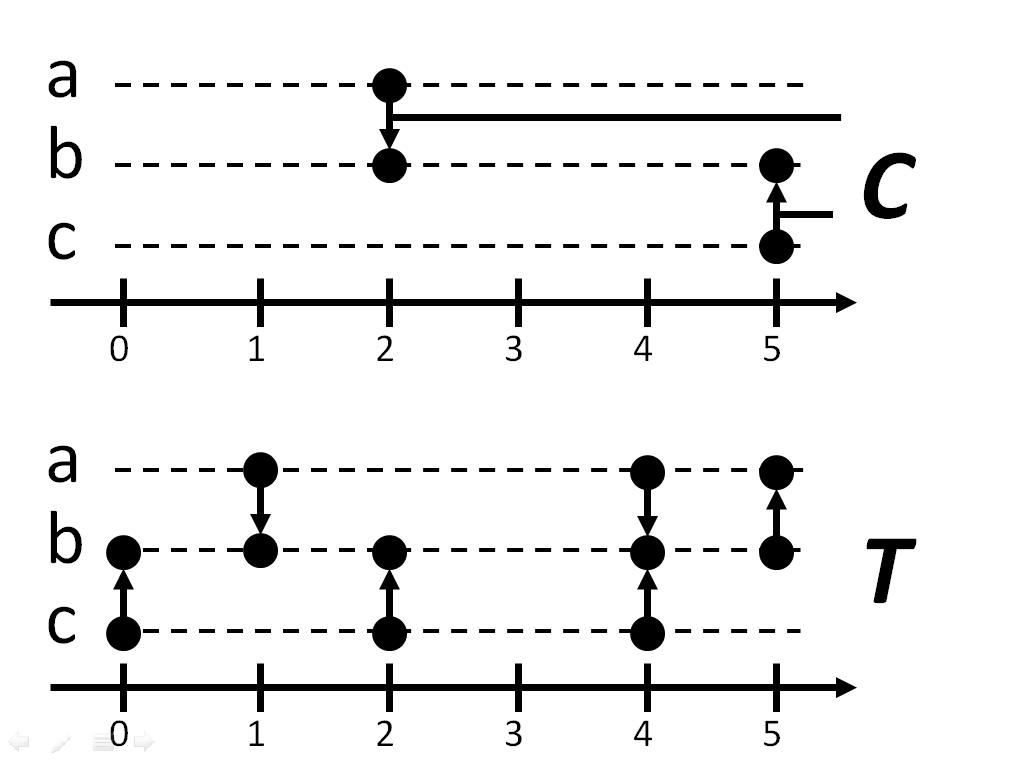
\includegraphics[width=.9\linewidth]{./figures/animation_dt/deltat-certif-0.png}}
			\only<2>{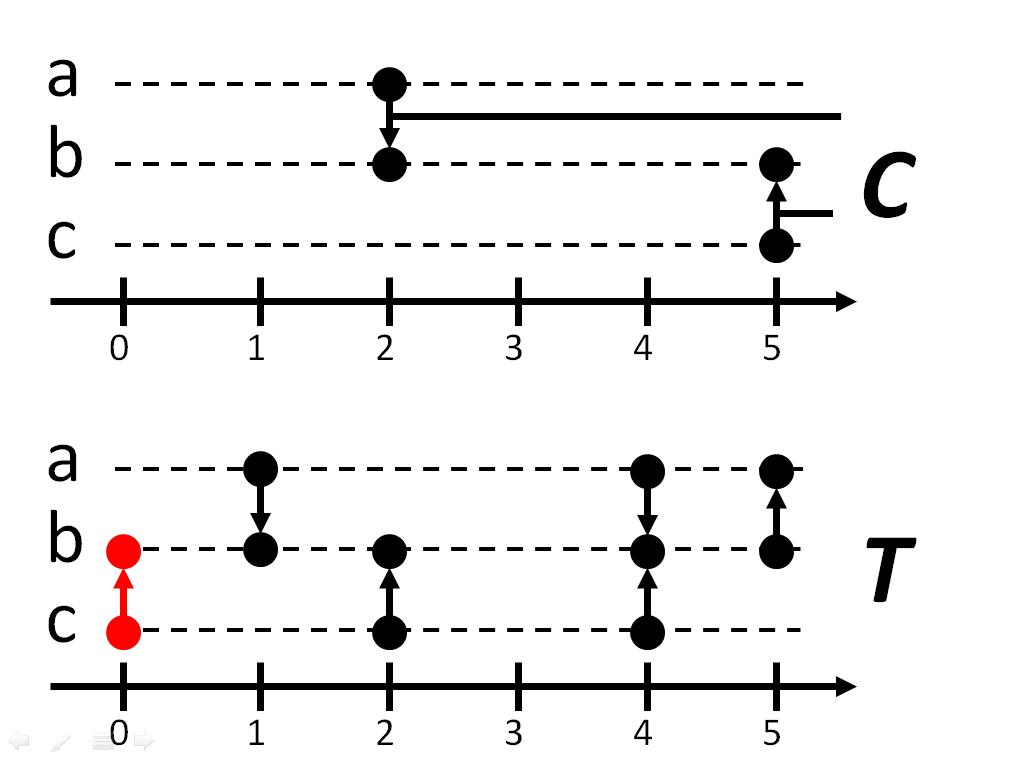
\includegraphics[width=.9\linewidth]{./figures/animation_dt/deltat-trans-1.png}}
			\only<3>{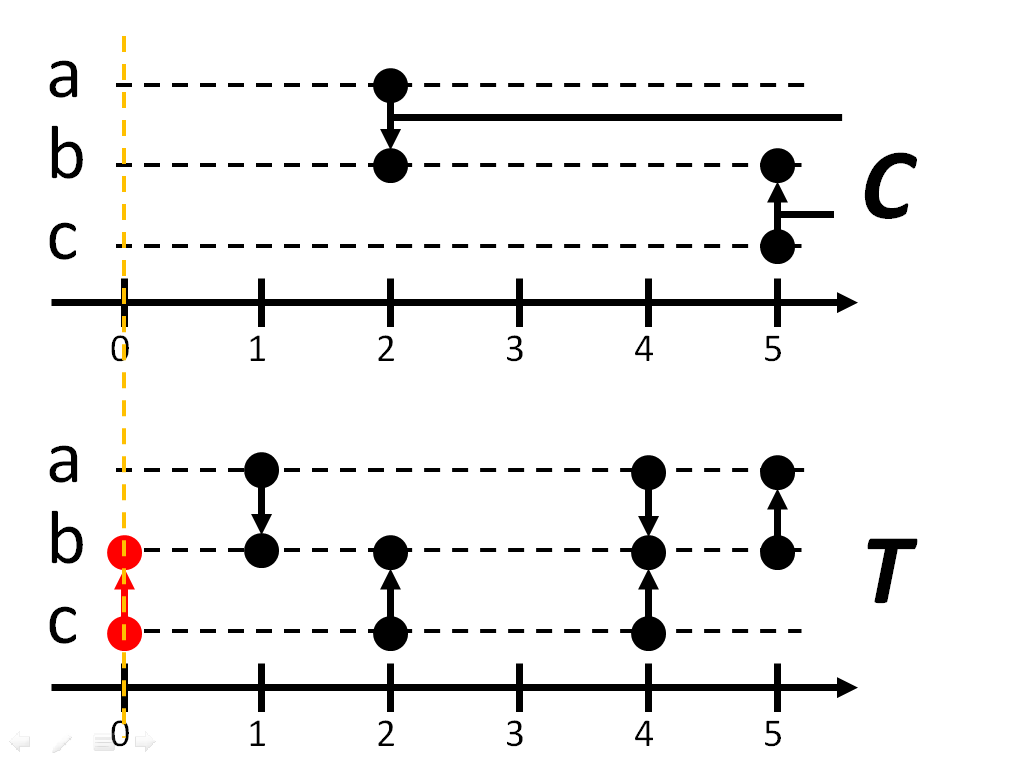
\includegraphics[width=.9\linewidth]{./figures/animation_dt/deltat-trans-2.png}}
			\only<4>{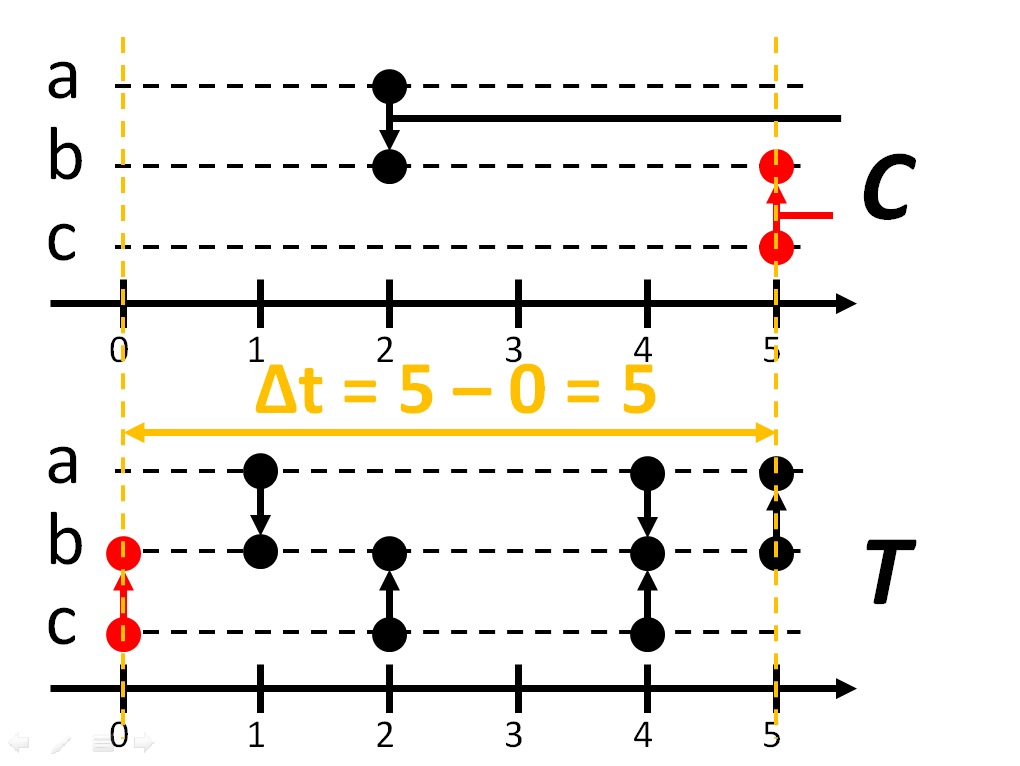
\includegraphics[width=.9\linewidth]{./figures/animation_dt/deltat-trans-3.png}}
		\end{figure}
	\end{center}
\end{frame}

%------------------------------------------------

\begin{frame}
	\frametitle{Time between transactions and certifications - \textbf{Results}}
	\begin{figure}
		\only<1>{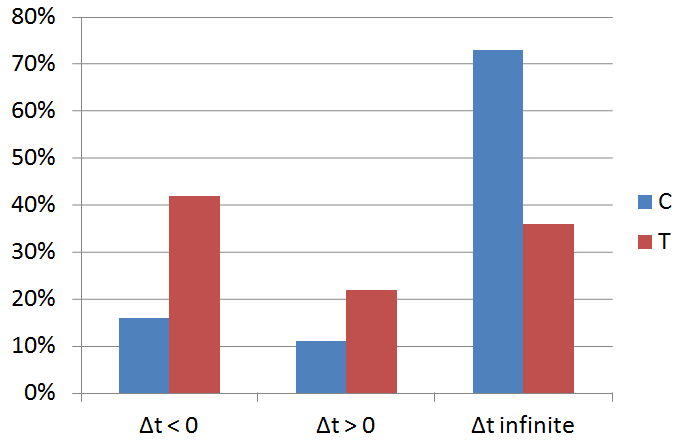
\includegraphics[width=.9\linewidth]{./figures/dt_distri}}
		\only<2>{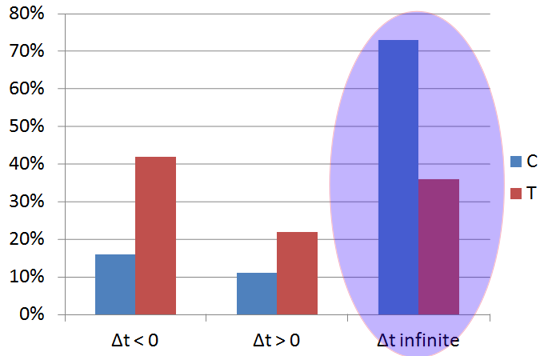
\includegraphics[width=.9\linewidth]{./figures/dt_distri_1}}
		\only<3>{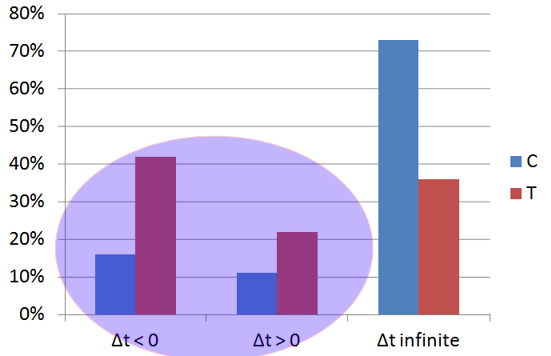
\includegraphics[width=.9\linewidth]{./figures/dt_distri_2}}
	\end{figure}
\end{frame}


%------------------------------------------------

\begin{frame}
	\frametitle{Time between transactions and certifications - \textbf{Results}}
	\begin{figure}
		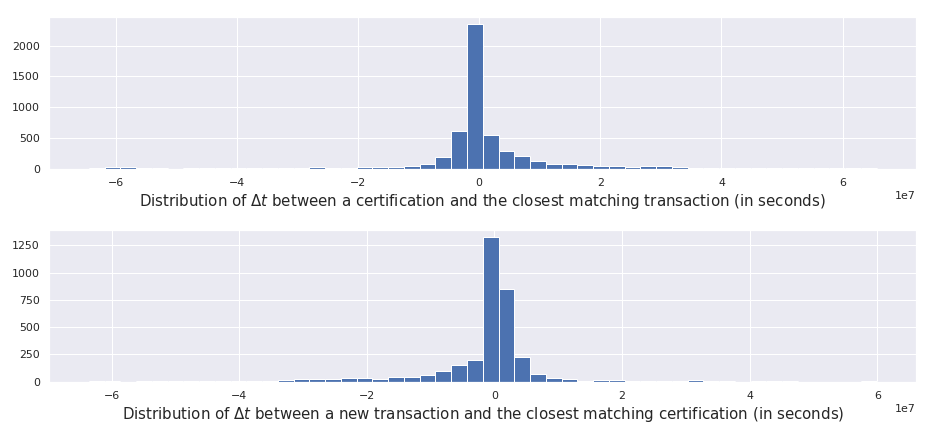
\includegraphics[width=\linewidth]{./figures/delta_t_simple}
	\end{figure}
\end{frame}

%------------------------------------------------
\subsection{Reciprocity and cycles}
%------------------------------------------------

\begin{frame}
	\frametitle{Reciprocity - \textbf{Questions}}
	{\Large \textbf{Questions:}}
	\begin{itemize}
		\item<1-> Are certifications/transactions reciprocal?
		\medskip
		\item<2-> How long does it take to get the opposite certification/transaction?
		\medskip
		\item<3-> How fast is the money cycling?
	\end{itemize}
\end{frame}

%------------------------------------------------

\begin{frame}
	\frametitle{Reciprocity - \textbf{K-Closures} of links - Ex: 2-closure}
	\begin{center}
		\begin{figure}
			\only<1>{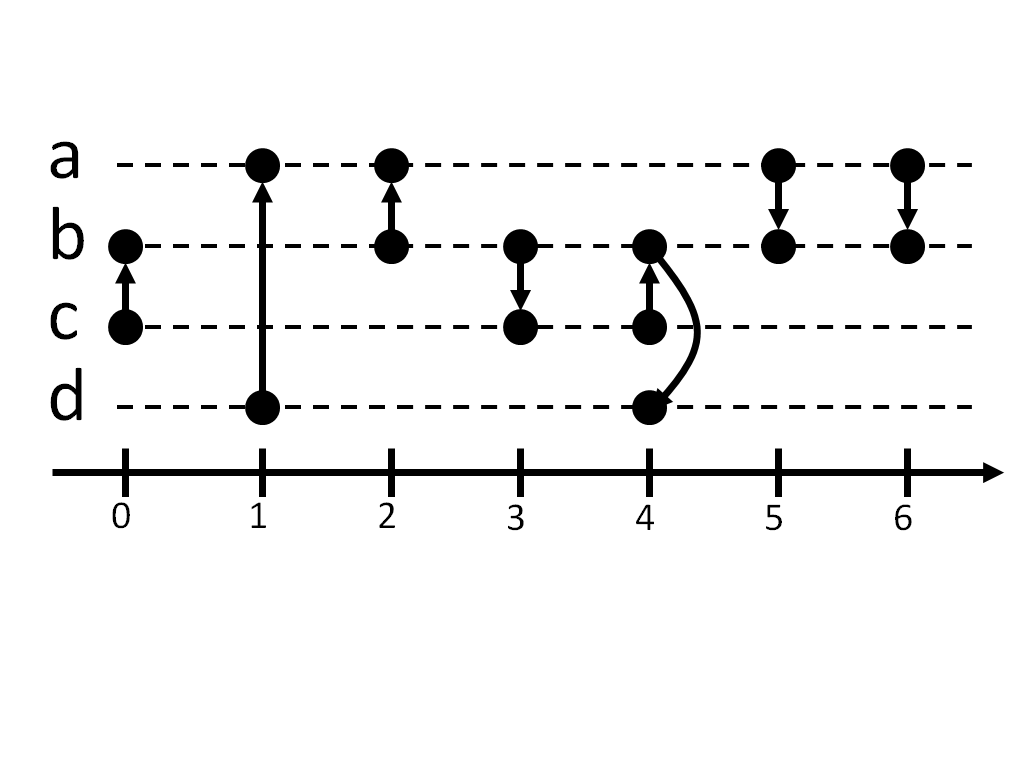
\includegraphics[width=\linewidth]{./figures/2-closure-0}}
			\only<2>{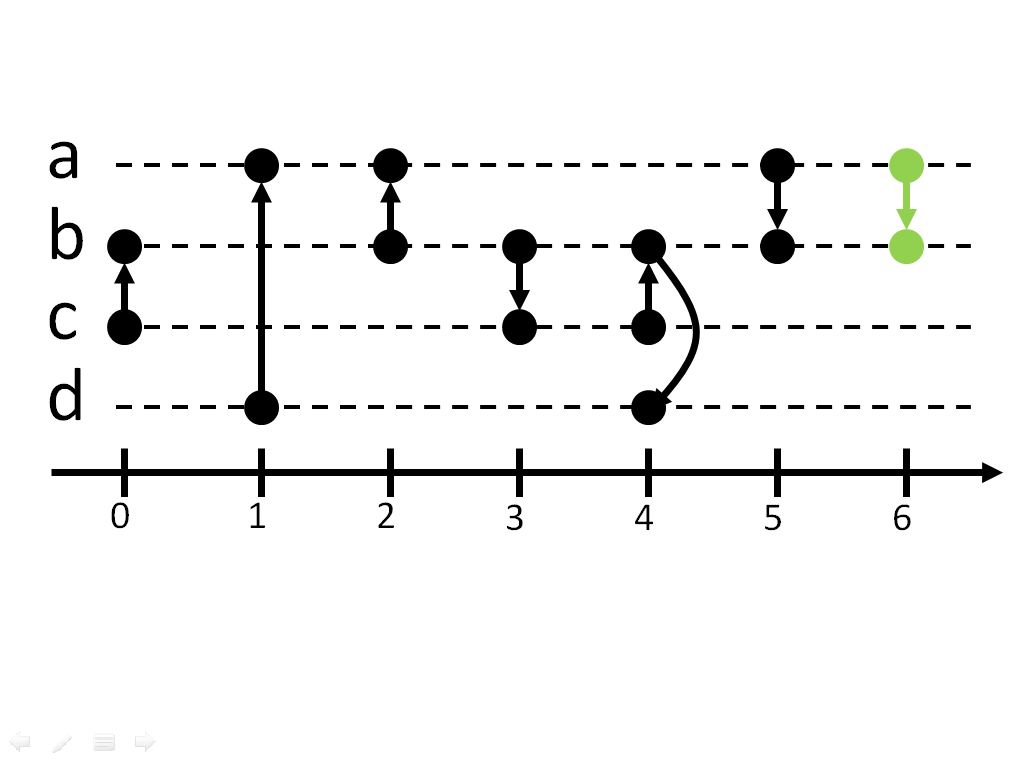
\includegraphics[width=\linewidth]{./figures/2-closure-1}}
			\only<3>{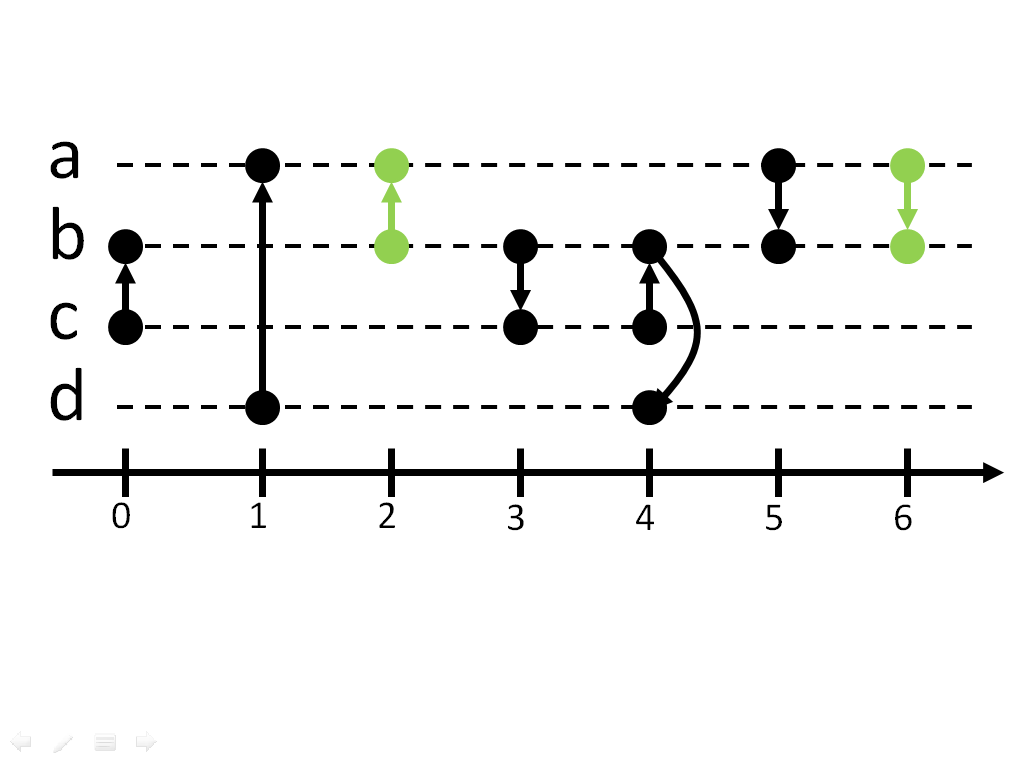
\includegraphics[width=\linewidth]{./figures/2-closure-2}}
			\only<4>{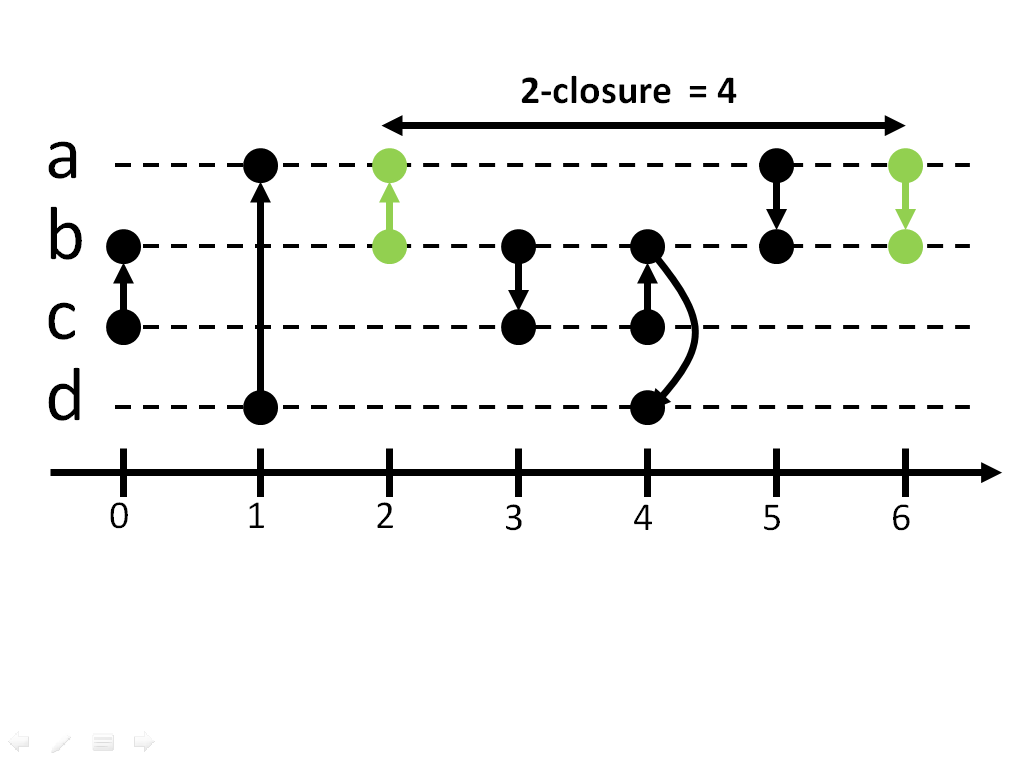
\includegraphics[width=\linewidth]{./figures/2-closure-3}}
		\end{figure}
	\end{center}
\end{frame}

%------------------------------------------------

\begin{frame}
	\frametitle{Reciprocity - \textbf{K-Closures} of links - Ex: 3-closure}
	\begin{center}
		\begin{figure}
			\only<1>{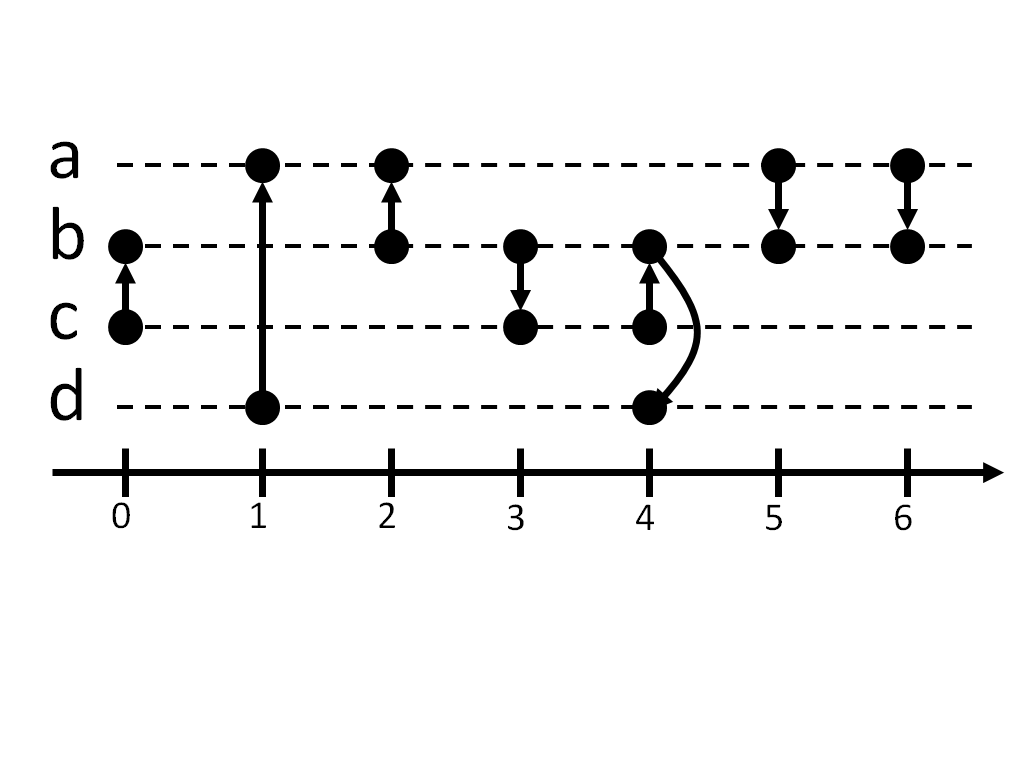
\includegraphics[width=\linewidth]{./figures/2-closure-0}}
			\only<2>{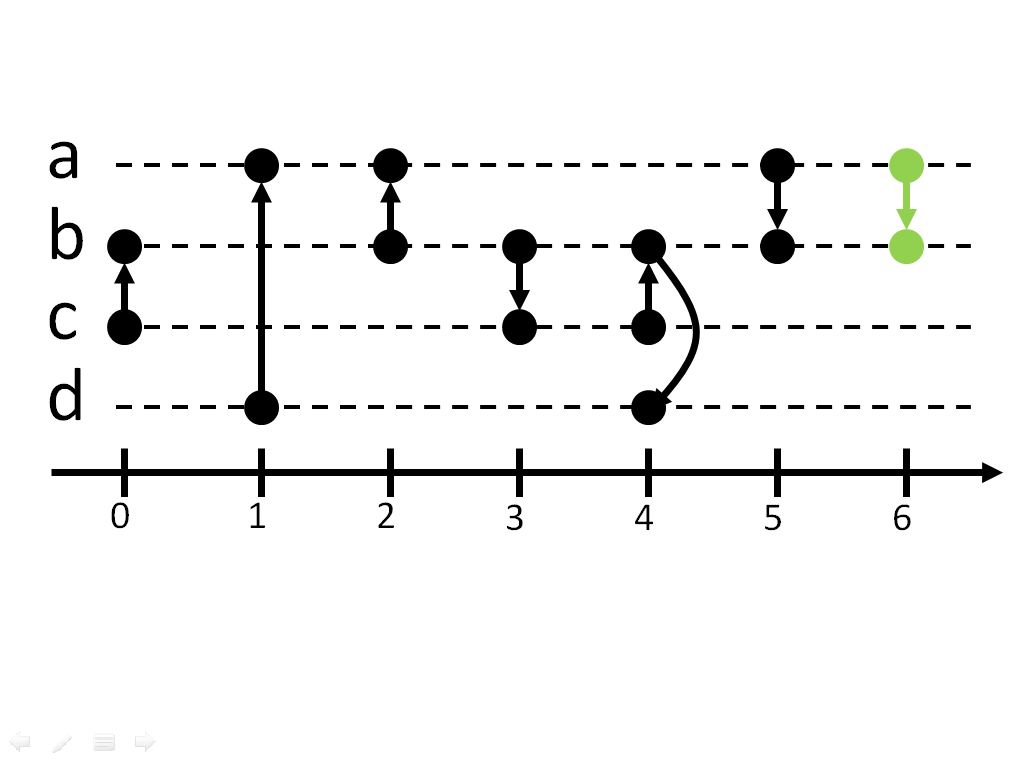
\includegraphics[width=\linewidth]{./figures/2-closure-1}}
			\only<3>{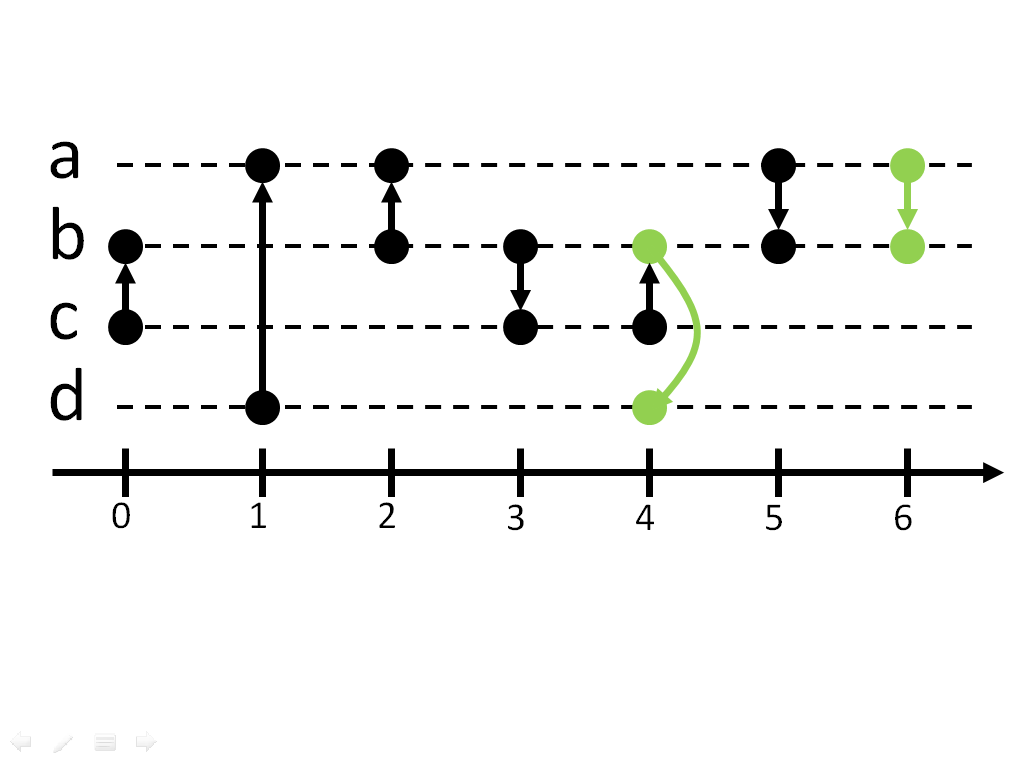
\includegraphics[width=\linewidth]{./figures/3-closure-2}}
			\only<4>{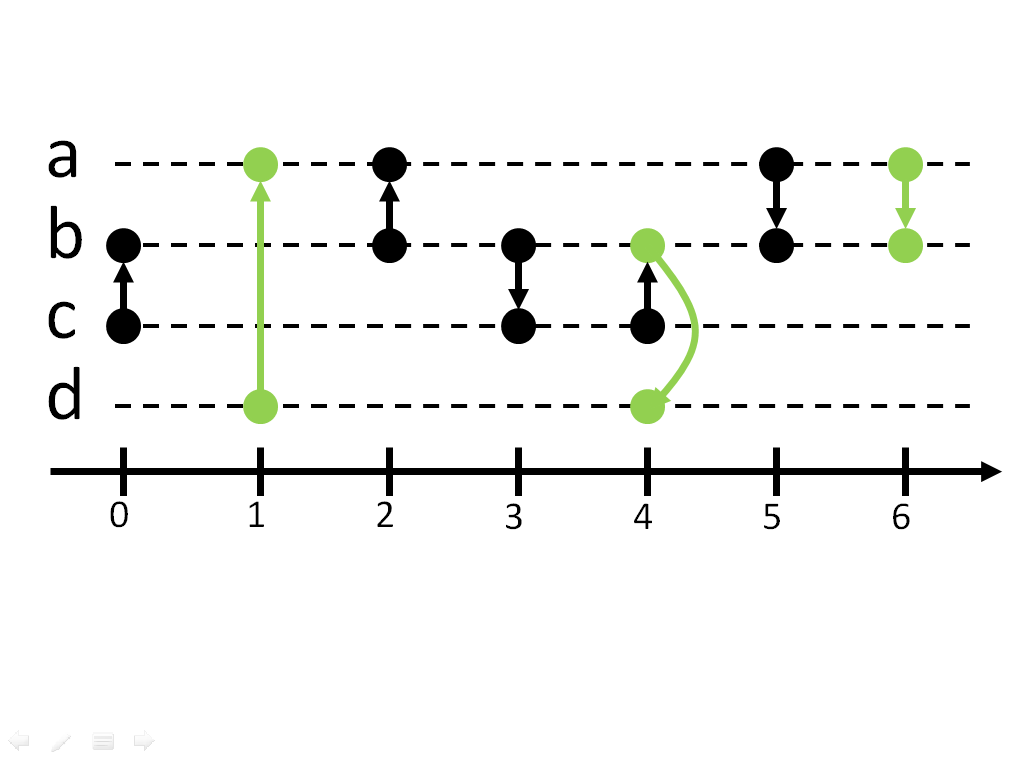
\includegraphics[width=\linewidth]{./figures/3-closure-3}}
			\only<5>{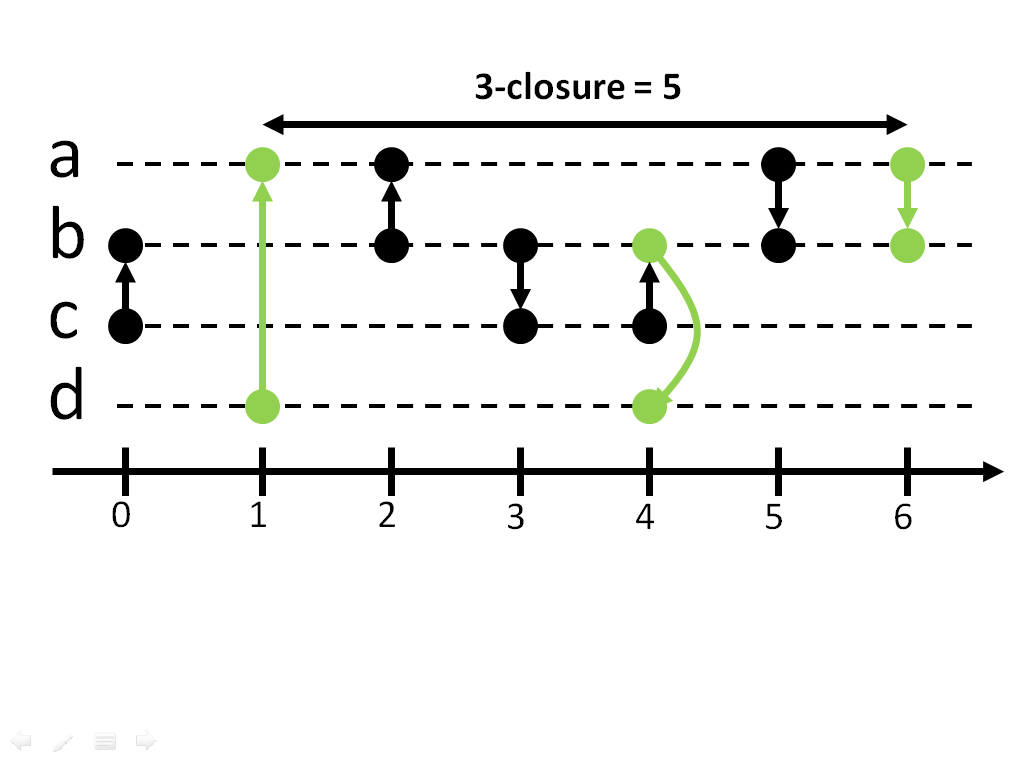
\includegraphics[width=\linewidth]{./figures/3-closure-4}}
		\end{figure}
	\end{center}
\end{frame}

%------------------------------------------------

\begin{frame}
	\frametitle{Reciprocity - \textbf{Results}}
	\begin{figure}
		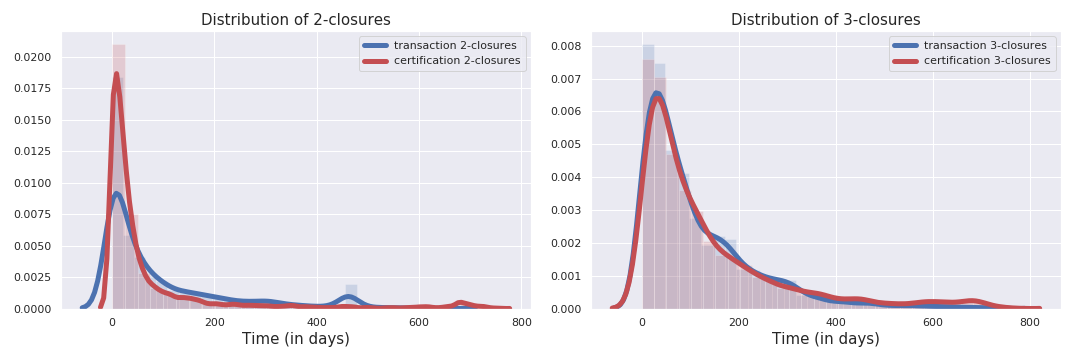
\includegraphics[width=\linewidth]{./figures/2-and-3-closures}
	\end{figure}
\end{frame}

%------------------------------------------------
\section{Conclusion}
%------------------------------------------------

\begin{frame}
	\frametitle{Conclusion and Takeaways}
	\begin{itemize}
		\item $\tilde{G}1$ offers a \textbf{unique dataset} to study the interplay between \textbf{social ties and transactions}
		\item The data is naturally well modeled by \textbf{stream graphs}
	\end{itemize}
	\medskip
	\begin{itemize}
		\item Members tend to certify people they never make transactions with
		\item But they tend to make transactions with people they are socially connected to
		\item When an interaction occurs in both streams, there is a clear time proximity
		\item Interactions tend to become reciprocal in short periods of time
	\end{itemize}
\end{frame}

%------------------------------------------------

\begin{frame}
	\Huge{\centerline{Questions?}}
	\bigskip
	{\normalsize Slides available on GitHub: \\ \textit{https://github.com/NicolasGensollen/presentation\_marami\_2019}}
	\bigskip	
	\begin{center}
	{\normalsize \textit{nicolas.gensollen@lip6.fr}}
	\end{center}
\end{frame}

%----------------------------------------------------------------------------------------

\end{document} 